%-----------------------------------------------------------------------------------------------------------------
% Modelo de documento para Disserta??o de Mestrado em Engenharia Electrot?cnica e de Computadores.
% Raul Morais, 2007 - 2008
% Manuel Cabral, 2008
%-----------------------------------------------------------------------------------------------------------------
\documentclass[12pt, twoside, a4paper, openright]{report}
\usepackage[centertags]{amsmath}
\usepackage{amsfonts}
\usepackage[portuguese]{babel}
\usepackage[utf8]{inputenc}           % Permite a escrita com acentos
\usepackage{amssymb}
\usepackage{amsthm}
\usepackage{amsmath}
\usepackage{newlfont}
\usepackage{fancyhdr}
\usepackage{graphicx}
\usepackage{natbib}
%\usepackage[dvips]{color}
\usepackage[dvipsnames]{xcolor}
\usepackage[rigidchapters]{titlesec}
\usepackage{mdwtab}
\usepackage{subfigure}
\usepackage{longtable}
\usepackage{UTADThesis} 
\usepackage{tabularx}
\usepackage{array}
\usepackage{diagbox}
\usepackage{slashbox,pict2e}\usepackage{makecell}

\usepackage{rotating}
\usepackage{tabularx}

\usepackage{wrapfig}

\usepackage{ragged2e}
\usepackage{lipsum}% for dummy text
\usepackage{floatrow}

\usepackage{algpseudocode}
\usepackage{titling}

\usepackage[final]{pdfpages}







% Definiçõees do template utilizado no MEEC/DEEC
\usepackage{url}                        % Tratamento dos endereços URL
\usepackage{makeidx}                    % Necess?rio para fazer o ?ndice remissivo
\usepackage{wrapfig}                    % Necess?rio para que o texto contorne as figuras
\usepackage{float}                      % Necess?rio para transcri??o de c?digo fonte
\usepackage{eurosym}                    % Necess?rio para se puder utilizar o s?mbolo oficial do Euro
\usepackage{array}                      % Necess?rio ? formata??o de tabelas
\usepackage{verbatim}
\usepackage{siunitx}

\usepackage[pdfauthor={Antonio Valente}, %
pdftitle={Modelo de documento para o MEEC/DEEC da UTAD},%
pagebackref=true,%
pdftex]{hyperref}
\usepackage{breakurl}

\hypersetup{
    colorlinks,%
    citecolor=red,%
    filecolor=red,%
    linkcolor=blue,%
    urlcolor=green,
    breaklinks=true
}

%-----------------------------------------------------------------------------------------------------------------
% Defini??es de espa?amentos e afins
%-----------------------------------------------------------------------------------------------------------------
\hfuzz2pt
\newlength{\defbaselineskip}
\setlength{\defbaselineskip}{\baselineskip}
\makeatletter
\renewcommand{\fnum@figure}[1]{\small\textbf{\figurename~\thefigure} -- \sffamily}%
\renewcommand{\fnum@table}[1]{\small\textbf{\tablename~\thetable} -- \sffamily} %
\makeatother
\makeatletter
\def\cleardoublepage{\clearpage\if@twoside \ifodd\c@page\else
\hbox{} \vspace*{\fill} \vspace{\fill} \thispagestyle{empty}
\newpage
\if@twocolumn\hbox{}\newpage\fi\fi\fi} \makeatother

\newcommand{\setlinespacing}[1]%
           {\setlength{\baselineskip}{#1 \defbaselineskip}}
\newcommand{\doublespacing}{\setlength{\baselineskip}%
                           {2.0 \defbaselineskip}}
\newcommand{\singlespacing}{\setlength{\baselineskip}{\defbaselineskip}}

\numberwithin{equation}{chapter}
\renewcommand{\theequation}{\thechapter.\arabic{equation}}
\setlength{\tclineskip}{1.05\baselineskip}

\newcommand\x[1]{\discretionary{#1}{#1}{#1}}

%-----------------------------------------------------------------------------------------------------------------
\setlength{\parindent}{0pt}            % Indenta??o de par?grafo
%-----------------------------------------------------------------------------------------------------------------
\makeindex                              % Necess?rio para o ?ndice Remissivo - Remover se n?o necess?rio
%-----------------------------------------------------------------------------------------------------------------
\floatstyle{ruled}                      % APAGAR AS 3 LINHAS
\newfloat{code}{thp}{lop}               % SE N?O NECESSITAR DE
\floatname{code}{Listagem}              % Necess?rio para utilizar listagens de c?digo-fonte
%-----------------------------------------------------------------------------------------------------------------
%\let ? = \euro                          % Permitir que se possa utilizar o s?mbolo directamente do teclado

%-----------------------------------------------------------------------------------------------------------------
%-------------------------------------------------------------------------
% Outros Termos e Comandos
%-------------------------------------------------------------------------
\newcommand{\LDC}{L_{\mathrm{DC}}}
\newcommand{\QL}{Q_{\mathrm{L}}}
\newcommand{\KVCO}{\mathrm{K}_{\mathrm{VCO}}}
\newcommand{\KPFD}{\mathrm{K}_{\phi}}
\newcommand{\UP}{\mathsf{UP}}
\newcommand{\DOWN}{\mathsf{DOWN}}
\newcommand{\NAND}{\mathsf{NAND}}

%\newcommand{\mi}[1]{#1\index{#1}}  % MARCA ENTRADA PARA O ÍNDICE REMISSIVO

%-------------------------------------------------------------------------
% Parâmetros MOSFET
%-------------------------------------------------------------------------
\newcommand{\GM}{g_{\mathrm{m}}}
\newcommand{\EOX}{\varepsilon_{\mathrm{OX}}}
\newcommand{\TOX}{\mathrm{t}_{\mathrm{OX}}}
\newcommand{\MOBILITYN}{\mu_{\mathrm{n}}}
\newcommand{\MOBILITYP}{\mu_{\mathrm{p}}}
\newcommand{\KPN}{\mathrm{KP}_{\mathrm{n}}}
\newcommand{\KPP}{\mathrm{KP}_{\mathrm{p}}}
\newcommand{\CDB}{C_{\mathrm{db}}}

%-------------------------------------------------------------------------
% Capacidades
%-------------------------------------------------------------------------
\newcommand{\COX}{C_{\mathrm{ox}}}
\newcommand{\CS}{C_{\mathrm{S}}}
\newcommand{\CB}{C_{\mathrm{B}}}

\newcommand{\RMS}{\mathrm{rms}}
\newcommand{\BW}{\mathrm{BW}}
\newcommand{\DS}{$\Delta\Sigma$ }
\newcommand{\MAX}{\mathrm{max}}
\newcommand{\SNRMAX}{\mathrm{SNR}_{\mathrm{max}}}
\newcommand{\SLEW}{\textit{slew-rate}}
%-------------------------------------------------------------------------
% Tempo e Frequência
%-------------------------------------------------------------------------
\newcommand{\TCLK}{T_{\mathrm{CLK}}}
\newcommand{\TN}{T_{\mathrm{N}}}
\newcommand{\TS}{T_{\mathrm{s}}}
\newcommand{\FS}{f_{\mathrm{s}}}
\newcommand{\FB}{f_{\mathrm{B}}}
\newcommand{\FN}{f_{\mathrm{N}}}
\newcommand{\FREF}{f_{\mathrm{REF}}}
\newcommand{\FDIV}{f_{\mathrm{DIV}}}
\newcommand{\FOUT}{f_{\mathrm{OUT}}}
\newcommand{\fout}{f_{\mathrm{out}}}
\newcommand{\fc}{f_{\mathrm{c}}}
\newcommand{\kbps}{\mathrm{kbps}}

%-------------------------------------------------------------------------
% Controlo de Espaços
%-------------------------------------------------------------------------
\newcommand{\EspacoPequeno}{\vskip2mm}
\newcommand{\EspacoMedio}{\vskip4mm}
\newcommand{\EspacoGrande}{\vskip8mm}
\newcommand{\EspacoExtra}{\vskip10mm}

%-------------------------------------------------------------------------
% Tensões
%-------------------------------------------------------------------------
\newcommand{\VOUT}{v_{\mathrm{out}}}
\newcommand{\VOUTMAX}{v_{\mathrm{out,max}}}
\newcommand{\VIN}{v_{\mathrm{in}}}
\newcommand{\VFB}{v_{\mathrm{FB}}}
\newcommand{\VFS}{V_{\mathrm{FS}}}
\newcommand{\VGS}{V_{\mathrm{GS}}}
\newcommand{\VP}{V_{\mathrm{P}}}
\newcommand{\VDS}{V_{\mathrm{DS}}}
\newcommand{\VDSON}{V_{\mathrm{DS,ON}}}
\newcommand{\vDSpico}{V_{\mathrm{DS,ON}}}
\newcommand{\VDD}{V_{\mathrm{DD}}}
\newcommand{\VSW}{v_{\mathrm{SW}}}
\newcommand{\VSWON}{V_{\mathrm{SW,ON}}}
\newcommand{\VCO}{\mathrm{VCO_{\mathrm{control}}}}
\newcommand{\VCP}{V_{\mathrm{CP}}}
\newcommand{\VRF}{V_{\mathrm{RF}}}
\newcommand{\GND}{\mathrm{GND}}

\newcommand{\VTN}{V_{\mathrm{TN}}}
\newcommand{\VTP}{V_{\mathrm{TP}}}
\newcommand{\VEFF}{V_{\mathrm{eff}}}
%-------------------------------------------------------------------------
% Correntes
%-------------------------------------------------------------------------
\newcommand{\ID}{I_{\mathrm{D}}}
\newcommand{\iD}{i_{\mathrm{D}}}
\newcommand{\iDpico}{i_{\mathrm{D,pico}}}
\newcommand{\IDC}{I_{\mathrm{DC}}}
\newcommand{\IDSS}{I_{\mathrm{DSS}}}
\newcommand{\ISW}{i_{\mathrm{SW}}}
\newcommand{\IRFMAX}{i_{\mathrm{RF,max}}}
\newcommand{\iRF}{i_{\mathrm{RF}}}
\newcommand{\IUP}{I_{\mathrm{UP}}}
\newcommand{\IDOWN}{I_{\mathrm{DOWN}}}
\newcommand{\IPUMP}{I_{\mathrm{pump}}}
\newcommand{\ICP}{I_{\mathrm{CP}}}
%-------------------------------------------------------------------------
% Potências
%-------------------------------------------------------------------------
\newcommand{\POUT}{P_{\mathrm{out}}}
\newcommand{\POUTMAX}{P_{\mathrm{out,max}}}
\newcommand{\PIN}{P_{\mathrm{in}}}
\newcommand{\PDC}{P_{\mathrm{DC}}}
%-------------------------------------------------------------------------
% Resistências
%-------------------------------------------------------------------------
\newcommand{\RL}{R_{\mathrm{L}}}
\newcommand{\ZIN}{Z_{\mathrm{in}}}
\newcommand{\ZOUT}{Z_{\mathrm{out}}}
\newcommand{\ZL}{Z_{\mathrm{L}}}
   % Carregar o ficheiro que contem macros e que ajudam na escrita
%-----------------------------------------------------------------------------------------------------------------
\begin{document}

%\nobib                                 % Op??es da Package UTADThesis - N?o apresenta as refer?ncias bibliogr?ficas
%\draft                                 % Op??es da Package UTADThesis - Vers?o draft do documento
%\nofront                               % Op??es da Package UTADThesis - N?o apresenta a parte frontal do doc
%\nojuri                                % Op??es da Package UTADThesis - N?o apresenta a descri??o do Juri

\renewcommand{\bibname}{Refer\^encias bibliogr\'aficas}
\renewcommand{\listtablename}{\'Indice de tabelas}
\renewcommand{\listfigurename}{\'Indice de figuras}
\renewcommand{\contentsname}{\'Indice geral}
\renewcommand{\indexname}{\'Indice remissivo}

\dedicate{ {\small "In the middle of difficulty lies opportunity" $\vert$ "No meio da dificuldade encontra-se a oportunidade."\\
            \bf{Einstein (1879 -- 1955)}}\\[1cm]
           {\small "Success is going from failure to failure without losing enthusiasm $\vert$ Sucesso é ir de fracasso em fracasso sem perder o entusiasmo"\\
            \bf{Winston Churchill(1874 -- 1965)}}\\[6cm]
   -% \begin{normalsize}
     %   A quem dedico,  \textbf{Nome}
    %\end{normalsize}\\%
    }%

%-----------------------------------------------------------------------------------------------------------------
%\nolistoftables                        % Op??es da Package UTADThesis - N?o apresenta o ?ndice de Tabelas
%\nolistoffigures                       % Op??es da Package UTADThesis - N?o apresenta o ?ndice de Figuras
%\msc                                    % Formato MasterOfScience
\phd									% Formato PhD
%-----------------------------------------------------------------------------------------------------------------
\title{Título da Dissertação-Tese\\Subtítulo se aplicável}
%-----------------------------------------------------------------------------------------------------------------
\author{Nome Completo do Aluno}
%-----------------------------------------------------------------------------------------------------------------
\orientador{Nome do Orientador 1}
\grauorientador{Professor Associado com Agregação}
\deporientador{Departamento de Engenharias}
\instorientador{Escola de Ciências e Tecnologia\\
da Universidade de Trás-os-Montes e Alto Douro}

\coorientador{Nome do Orientador 2}
\graucoorientador{Professor Auxiliar}
\depcoorientador{Departamento de Engenharias}
\instcoorientador{Escola de Ciências e Tecnologia\\
da Universidade de Trás-os-Montes e Alto Douro
}

\begin{figure}[h]
    \centering
    
\includegraphics[width=0.2\textwidth]{Acessorios/UTAD.JPG}
    \label{fig:blocos}  
\end{figure}
%-----------------------------------------------------------------------------------------------------------------
% Indica??o dos elementos do acompanhante do trabalho - Apenas se existir
%-----------------------------------------------------------------------------------------------------------------
%\acompanhante{}
%\grauacompanhante{l}
%\depacompanhante{l}
%\instacompanhante{l\\
               %  l}
%-----------------------------------------------------------------------------------------------------------------
% Indicação dos elementos do Presidente do Júri
%-----------------------------------------------------------------------------------------------------------------
\presidentejuri{Nome Presidente do Júri}
\designacaopresidente{Direção do Mestrado em Engenharia Eletrotecnica e de Computadores do Departamento de Engenharias da Universidade de Trás-os-Montes e Alto Douro}
%-----------------------------------------------------------------------------------------------------------------
% Indicação dos elementos do Arguente do trabalho
%-----------------------------------------------------------------------------------------------------------------
\arguenteexterno{Doutor João Paulo Coelho}
\designacaoarguente{Professor Adjunto da Escola Superior de Tecnologia e Gestão do Instituto Politécnico de Bragança}
%-----------------------------------------------------------------------------------------------------------------


\beforepreface
%-----------------------------------------------------------------------------------------------------------------
\pagestyle{plain} %
%-----------------------------------------------------------------------------------------------------------------
\phantomsection
\addcontentsline{toc}{chapter}{Resumo}
%-----------------------------------------------------------------------------------------------------------------
% Resumo em Português
%-----------------------------------------------------------------------------------------------------------------


\begin{center}
\large{Título}

\vskip5mm
\normalsize{\textit{Autor}}


\vskip5mm
\small{Submetido na Universidade de Trás-os-Montes e Alto Douro \\
para o preenchimento dos requisitos parciais para obtenção do grau de \\
Mestre/Doutor em Engenharia Electrotécnica e de Computadores}
\end{center}

\textbf{Resumo ---} 
Ius wisi imperdiet et, vis ea inimicus dissentias. Has dicit luptatum cu. Accumsan patrioque sea ea. Est ea viderer dissentiet, sit ad tempor oporteat, per causae volumus patrioque id. At pri debet vocent honestatis, postulant disputationi at mei.

Assum erant dolorem an has, odio eripuit an sit, no enim meis malis eam. Ex possim utamur prompta sea. Vocibus verterem cum id, et ubique virtute detraxit mel. Usu ex esse quot, in est quot inani docendi. Prima mollis cu usu, ad sumo probo summo mea. Laudem omittantur ut mea.

\textbf{Palavras Chave:} Palavra1, Palavra2, Palavra3.

%-----------------------------------------------------------------------------------------------------------------

%-----------------------------------------------------------------------------------------------------------------
\cleardoublepage
\phantomsection
\addcontentsline{toc}{chapter}{\textit{Abstract}}
%-----------------------------------------------------------------------------------------------------------------
% Abstract - Resumo em Inglês
%-----------------------------------------------------------------------------------------------------------------

\begin{center}
\large{Title}

\vskip5mm
\normalsize{\textit{Author Name}}

\vskip5mm
\small{Submitted to the University of Trás-os-Montes and Alto Douro \\
in partial fulfillment of the requirements for the degree of \\
Master of Science-Philosophiae Doctor in Electrical Engineering and Computers}
\end{center}

\textbf{Abstract ---} 
Lorem ipsum dolor sit amet, sed ex nonumes omittam ponderum, sea ut adipiscing inciderint. Vidisse delenit vel ad. Ei nec eripuit deseruisse, ex eos esse maiestatis. Modo vocent lobortis pri id, wisi habemus percipitur ei sit, eu nec cibo quidam dictas. Illum vivendum sed ex.

Et vis assum meliore, quod vide contentiones qui an, postea semper sit no. Ei erant democritum accommodare mel, ut aeque senserit vim. Cum ne essent voluptua, no vix ferri labores. Eam id essent eruditi sensibus, in etiam dicit ridens eos, veri offendit imperdiet has ad. Integre salutatus eu pro, has ei denique senserit.

\textbf{Key Words: Word1, Word2, Word3} 

%-----------------------------------------------------------------------------------------------------------------

%-----------------------------------------------------------------------------------------------------------------
\phantomsection
%-----------------------------------------------------------------------------------------------------------------
\prefacesection{Agradecimentos}
%-----------------------------------------------------------------------------------------------------------------
Meis summo ex eam, facer animal voluptaria te quo. Ad vix ancillae reprehendunt, mei integre erroribus te, eum aliquam platonem corrumpit ex. Pri tractatos definiebas ex, per alii zril diceret ea. Te per purto nulla scripta, dolorum facilis eam ea, autem dicant putent ex vis. Ad sed prima ipsum, ex cum alia simul.

In mel equidem verterem, dicta gloriatur definitionem eos ad. Mel id nulla inermis. Sed placerat reformidans at. Nibh eius eu vix, cum dolore eripuit evertitur eu, at velit phaedrum sed. At eum erant aperiri mediocrem, ius inani disputando ex. Usu aliquid moderatius disputationi te, dico ornatus moderatius an mei.

Per affert conclusionemque no. Quo et dico mazim vivendum, id senserit repudiare efficiantur vix, pri at consequat adversarium. Te quem mandamus qui, an enim laudem sed. An has omnis summo eleifend, ei sed eripuit similique.

Inani legimus constituam pri no, ullum blandit gubergren ne mel. Sea an vivendo fierent. Debitis nusquam definiebas in mea, nec ea viris moderatius. Eam te idque deterruisset, eum elit malorum maiorum no, usu id omnes appareat vituperata. Omnis dicat iuvaret ea sea, et alii alterum nec. Congue comprehensam eu sed.

Viris tempor no eos, has ex causae percipit iracundia, per id platonem inciderint. Ex omnis iusto fastidii mei. Id mea sint tempor. Te idque epicuri pri, at homero regione mel, eam nostrud fabellas facilisis no. At veri molestiae mediocritatem quo, eu accusamus maiestatis scribentur sit, wisi disputando ex pri. An bonorum complectitur sed, ignota petentium ei qui, vidisse salutatus cu per.

Sea ad duis quaeque euripidis, id duo primis facete denique. An nulla iusto tation vix. Duis prompta assentior et his, ut ius tollit aliquid. Tamquam blandit mel an, vim cu quas dicat, eam eu magna dictas.


\EspacoMedio
\EspacoMedio
\EspacoMedio
\noindent UTAD, \hfill Nome \\ Vila Real, xx de xxxxx de 20XX
%-----------------------------------------------------------------------------------------------------------------

%-----------------------------------------------------------------------------------------------------------------
\cleardoublepage
\phantomsection
\currentpdfbookmark{\contentsname}{}
\tableofcontents%
%-----------------------------------------------------------------------------------------------------------------
\cleardoublepage
\phantomsection
\addcontentsline{toc}{chapter}{\listtablename}
%\listoftables %
%-----------------------------------------------------------------------------------------------------------------
\cleardoublepage
\phantomsection
\addcontentsline{toc}{chapter}{\listfigurename}
\listoffigures%
%-----------------------------------------------------------------------------------------------------------------
%-----------------------------------------------------------------------------------------------------------------
% Glossário de termos, lista de acrónimos e lista de abreviaturas
%-----------------------------------------------------------------------------------------------------------------
\prefacesection{Glossário, acrónimos e abreviaturas}
{
    \setlinespacing{1.33}
    \def\baselinestretch{1.15}
    \renewcommand{\arraystretch}{1.1}
    \setlength{\arrayrulewidth}{0.2mm}%
%-----------------------------------------------------------------------------------------------------------------
\section*{Glossário de termos}
%-----------------------------------------------------------------------------------------------------------------
\vskip10mm

%-----------------------------------------------------------------------------------------------------------------
\section*{Lista de acrónimos}
%-----------------------------------------------------------------------------------------------------------------

\begin{longtable}[c]{p{3cm} p{11cm}}
    \textbf{Sigla} & \textbf{Expansão} \\
    \endfirsthead
    \textbf{Sigla} & \textbf{Expansão} \\
    \endhead
    \endfoot
    \endlastfoot\\
    CMOS & \textit {Complementary Metal-Oxide-Semiconductor} \\
    DC & \emph{Direct Current} (corrente contínua) \\
    
    MOSFET & \textit {Metal-Oxide-Semiconductor Field-Effect Transistor} \\
    
\end{longtable}

\vskip20mm
%-----------------------------------------------------------------------------------------------------------------

%-----------------------------------------------------------------------------------------------------------------



%-----------------------------------------------------------------------------------------------------------------

%-----------------------------------------------------------------------------------------------------------------
\afterpreface
%-----------------------------------------------------------------------------------------------------------------
\setlength{\parskip}{10pt}                  % Salto de par?grafo
\def\baselinestretch{1.15}
%-----------------------------------------------------------------------------------------------------------------
%----------------------------------------------------------

-------------------------------------------------------
\chapter{Introdução}
\label{Ch:Introducao}
%---------------------------------------------------------------------------------------------------------------
Lorem ipsum dolor sit amet, sed ex nonumes omittam ponderum, sea ut adipiscing inciderint. Vidisse delenit vel ad. Ei nec eripuit deseruisse, ex eos esse maiestatis. Modo vocent lobortis pri id, wisi habemus percipitur ei sit, eu nec cibo quidam dictas. Illum vivendum sed ex~\ref{Fig:FigExample}.

Et vis assum meliore, quod vide contentiones qui an, postea semper sit no. Ei erant democritum accommodare mel, ut aeque senserit vim. Cum ne essent voluptua, no vix ferri labores. Eam id essent eruditi sensibus, in etiam dicit ridens eos, veri offendit imperdiet has ad. Integre salutatus eu pro, has ei denique senserit.

Meis summo ex eam, facer animal voluptaria te quo. Ad vix ancillae reprehendunt, mei integre erroribus te, eum aliquam platonem corrumpit ex. Pri tractatos definiebas ex, per alii zril diceret ea. Te per purto nulla scripta, dolorum facilis eam ea, autem dicant putent ex vis. Ad sed prima ipsum, ex cum alia simul.
Tania Macedo~\citep{Rules};~\citep{7886612}
(\citeauthor{Rules}, \citeyear{Rules}; \citeauthor{7886612},\citeyear{7886612})



\begin{figure}
\centering
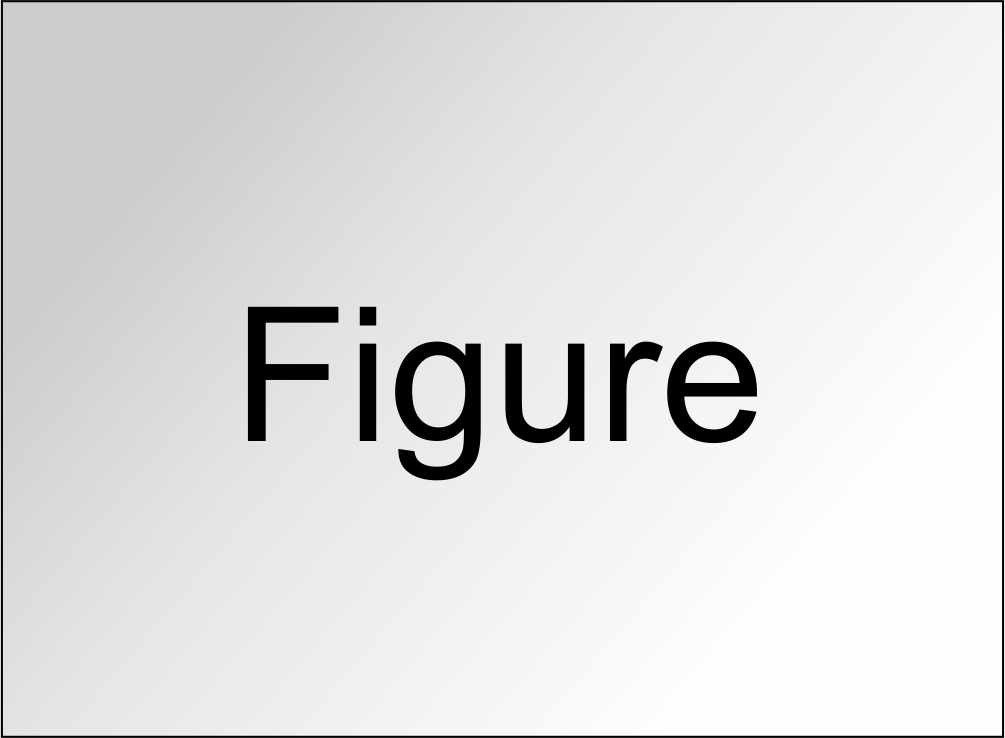
\includegraphics[width=0.7\linewidth]{Cap1/Figure.jpg} 
\caption{Figure Example}
\label{Fig:FigExample}
\end{figure}

%-----------------------------------------------------------------------------------------------------------------
\section{Motivação e objectivos}
%-----------------------------------------------------------------------------------------------------------------

In mel equidem verterem, dicta gloriatur definitionem eos ad. Mel id nulla inermis. Sed placerat reformidans at. Nibh eius eu vix, cum dolore eripuit evertitur eu, at velit phaedrum sed. At eum erant aperiri mediocrem, ius inani disputando ex. Usu aliquid moderatius disputationi te, dico ornatus moderatius an mei.

Per affert conclusionemque no. Quo et dico mazim vivendum, id senserit repudiare efficiantur vix, pri at consequat adversarium. Te quem mandamus qui, an enim laudem sed. An has omnis summo eleifend, ei sed eripuit similique.

Inani legimus constituam pri no, ullum blandit gubergren ne mel. Sea an vivendo fierent. Debitis nusquam definiebas in mea, nec ea viris moderatius. Eam te idque deterruisset, eum elit malorum maiorum no, usu id omnes appareat vituperata. Omnis dicat iuvaret ea sea, et alii alterum nec. Congue comprehensam eu sed.



%-----------------------------------------------------------------------------------------------------------------
\section{Organização da dissertação}
%-----------------------------------------------------------------------------------------------------------------

Viris tempor no eos, has ex causae percipit iracundia, per id platonem inciderint. Ex omnis iusto fastidii mei. Id mea sint tempor. Te idque epicuri pri, at homero regione mel, eam nostrud fabellas facilisis no. At veri molestiae mediocritatem quo, eu accusamus maiestatis scribentur sit, wisi disputando ex pri. An bonorum complectitur sed, ignota petentium ei qui, vidisse salutatus cu per.

Sea ad duis quaeque euripidis, id duo primis facete denique. An nulla iusto tation vix. Duis prompta assentior et his, ut ius tollit aliquid. Tamquam blandit mel an, vim cu quas dicat, eam eu magna dictas.

Ius wisi imperdiet et, vis ea inimicus dissentias. Has dicit luptatum cu. Accumsan patrioque sea ea. Est ea viderer dissentiet, sit ad tempor oporteat, per causae volumus patrioque id. At pri debet vocent honestatis, postulant disputationi at mei.

Assum erant dolorem an has, odio eripuit an sit, no enim meis malis eam. Ex possim utamur prompta sea. Vocibus verterem cum id, et ubique virtute detraxit mel. Usu ex esse quot, in est quot inani docendi. Prima mollis cu usu, ad sumo probo summo mea. Laudem omittantur ut mea.

%-----------------------------------------------------------------------------------------------------------------

%-----------------------------------------------------------------------------------------------------------------
%-----------------------------------------------------------------------------------------------------------------
\chapter{Título do Capítulo 1}
\label{Ch:EstadoDaArte}
%-------------------------------------------------------------------------------------------------------------
Exemplo de utilização no sistema de unidades SI~\SI{2}{\min} \SI{27}{\second} e de referências no texto~\citep{Rules}~\citep{AllJapan}.

 







%-----------------------------------------------------------------------------------------------------------------


%-----------------------------------------------------------------------------------------------------------------
%-------------------------------------------------------------------------


\chapter{Outro Capítulo}
\label{Ch:OutroCap}
%------------------------------------------------------------------------------------------------------------

%-----------------------------------------------------------------------------------------------------------------
%-----------------------------------------------------------------------------------------------------------------
\chapter[Título para o Índice]{Título para figurar no corpo da tese/dissertação}
\label{Ch:CapExemplo}




%-----------------------------------------------------------------------------------------------------------------
%-----------------------------------------------------------------------------------------------------------------
\chapter[Resultados]{Resultados}
\label{Ch:Resultados}

Exemplo de um algorítmo
\begin{algorithmic}[1]
\State $LeituraEscuro \gets Leitura da ADC antes do LED emissor ligar$
	\State $LeituraLuz \gets Leitura da ADC depois do LED emissor ligar$ 
    \State $LeituraReal \gets Leitura correta do valor dos sensores$ 
    \State $Limit \gets Valorda ADC para o qual se considera proximidade da parede$ 
\Repeat
\State $LeituraEscuro \gets LerADC$
\State $LEDEmissor \gets ON$
\State $LeituraLuz \gets LerADC$
\State $LEDEmissor \gets OFF$
\State $LeituraReal \gets LeituraLuz - LeituraEscuro$

\If {$LeituraReal < Limit$}
    \State \Return $Nao ha parede$
  \Else
    \State \Return $Ha parede$
  \EndIf

\Until{$TodosSensoresLidos$}

\end{algorithmic}





%-----------------------------------------------------------------------------------------------------------------

%-----------------------------------------------------------------------------------------------------------------

%-----------------------------------------------------------------------------------------------------------------
\chapter[Conclusão e trabalho futuro]{Conclusão e trabalho futuro}
\label{Ch:Conclusao}

 


%-----------------------------------------------------------------------------------------------------------------

%GATHER{MyBibDataBase.bib}                  % Não mexer nesta linha - Comando WinEdt
\cleardoublepage
\bibliographystyle{apa}                  % Formato IEEE Transactions
\nocite{*}                                  % Lista toda a bibliografia do ficheiro bib
\phantomsection
\bibliography{MyBibDataBase}
%-----------------------------------------------------------------------------------------------------------------
% Depois da bibliografia, vêm os anexos (Letras)
%-----------------------------------------------------------------------------------------------------------------
\appendix
%-----------------------------------------------------------------------------------------------------------------
\cleardoublepage
% ------------------------------------------------------------------
% Parâmetros do Processo AMI C07MA
% ------------------------------------------------------------------

\chapter{Apêndice}


\section*{Datasheets}



\subsection{DS3231}
\newcommand*\side{90}

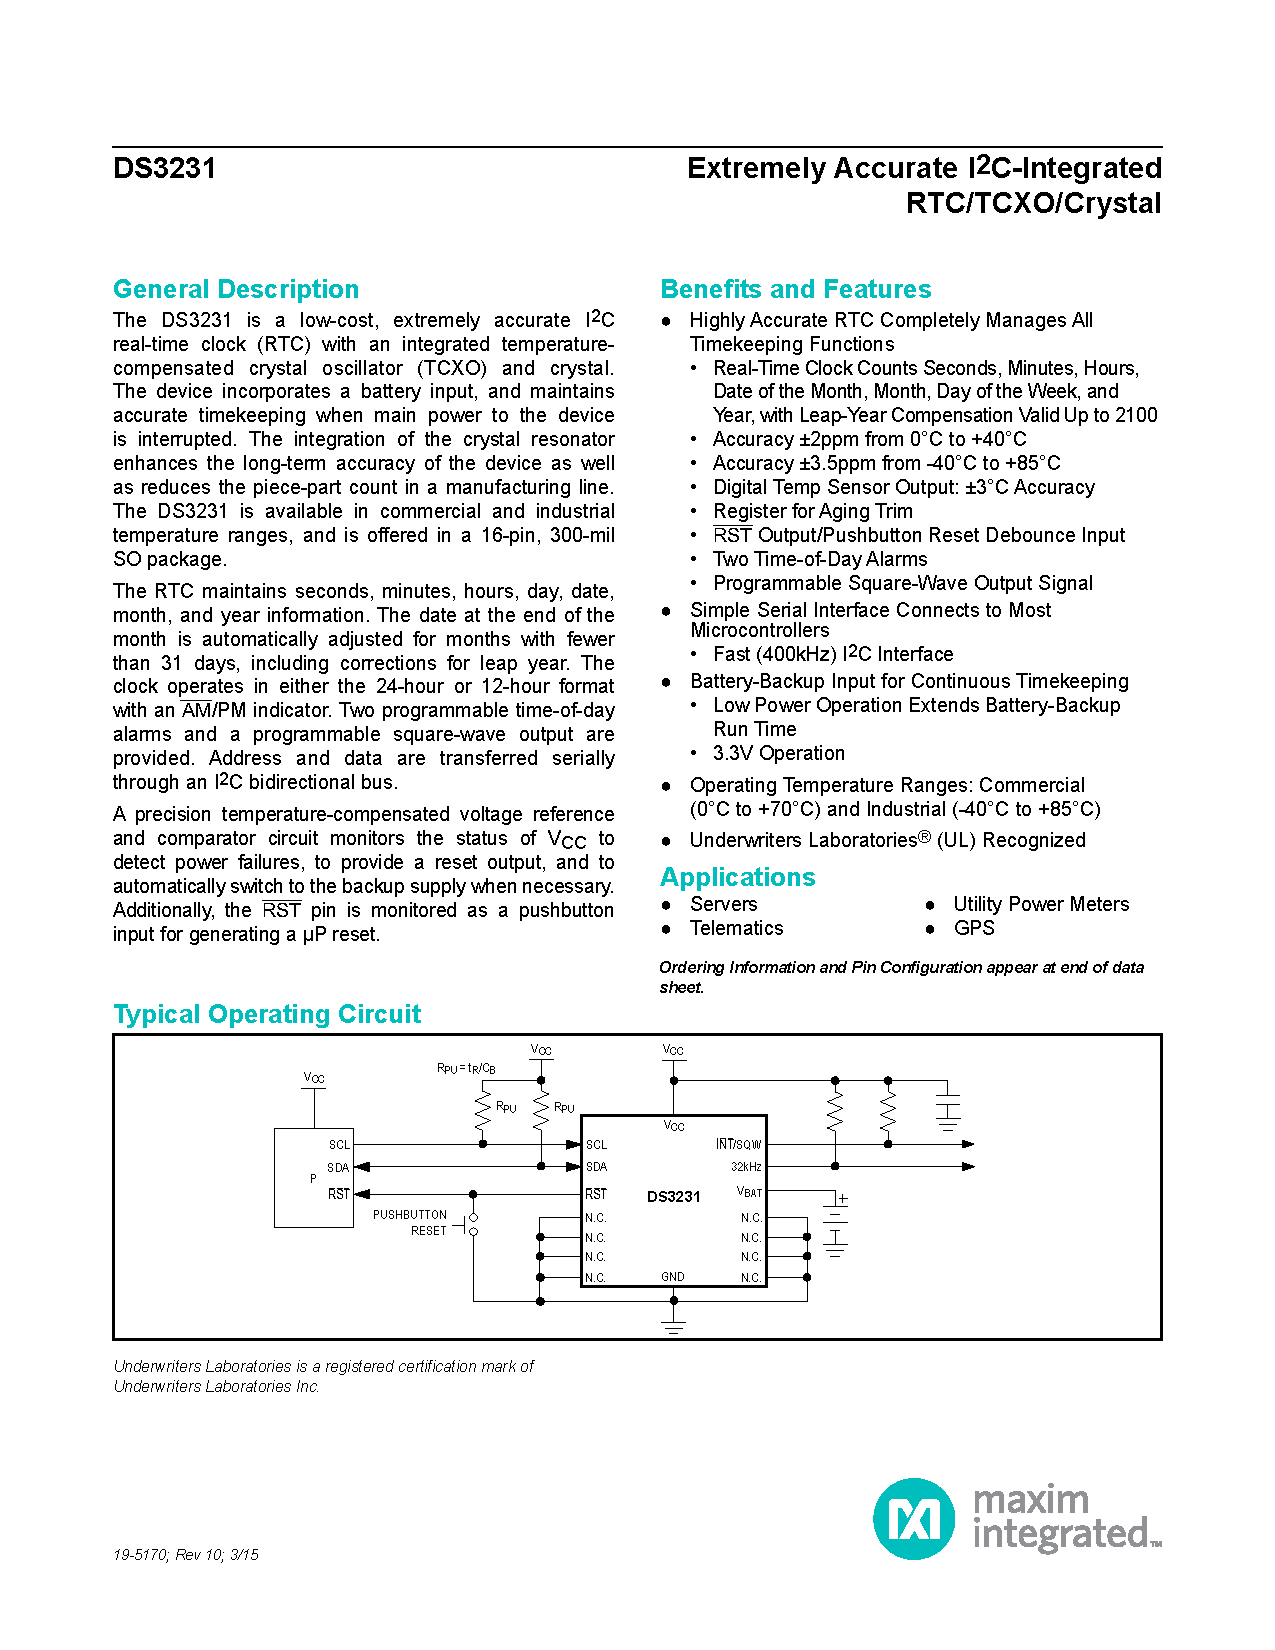
\includepdf[pages=-,width=\textwidth,pagecommand={\xdef\side{\the\numexpr-\side\relax}}]{Acessorios/datasheet.pdf}

% ---------------------------------------------------------------------

%-----------------------------------------------------------------------------------------------------------------
\cleardoublepage
\include{Acessorios/MyAppendixB}
%-----------------------------------------------------------------------------------------------------------------
\cleardoublepage
\phantomsection
\addcontentsline{toc}{chapter}{\indexname}
\printindex                                 % Imprime o ?ndice remissivo (N?o esquecer compilar com MakeIndex)
%-----------------------------------------------------------------------------------------------------------------
\cleardoublepage
%\include{Acessorios/MySobreOAutor}          % Imprimir informa??osobre o Autor
%-----------------------------------------------------------------------------------------------------------------
\end{document}
%-----------------------------------------------------------------------------------------------------------------
